% ===================================================================
%  Αρχείο: 15191_tikz.tex (Fragment)
%  Αυτόματη μετατροπή μέσω doc2latex.py & TikZ conversion
% ===================================================================

ΘΕΜΑ 2

Στο διπλανό σχήμα δίνεται ο τριγωνομετρικός κύκλος, μια γωνία $x\widehat{O}A = \omega$ και η τελική της πλευρά τέμνει τον κύκλο στο σημείο $Μ(-0.8, y)$.

\begin{alist}
\item Με βάση το σχήμα:
\begin{rlist}
\item να βρείτε το συνημίτονο της γωνίας $\omega$.

\monades{4}

\item να αιτιολογήσετε γιατί $\eta\mu\omega > 0$.

\monades{8}
\end{rlist}
\item \monades{13} Να υπολογίσετε το ημίτονο της γωνίας $\omega$.

\begin{center}
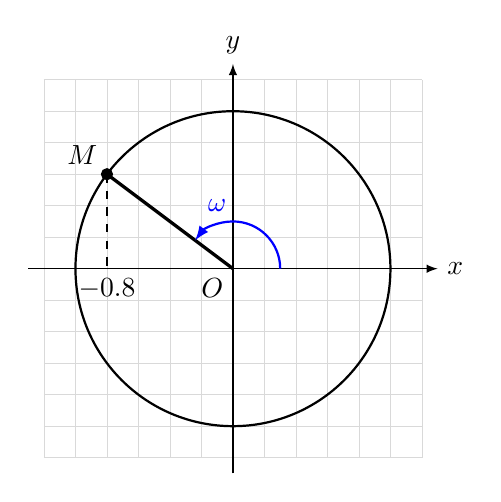
\begin{tikzpicture}[scale=2, >=latex]
    \draw[very thin, color=gray!30, step=0.2] (-1.2,-1.2) grid (1.2,1.2);
    \draw[thick] (0,0) circle (1);
    \draw[->] (-1.3,0) -- (1.3,0) node[right] {$x$};
    \draw[->] (0,-1.3) -- (0,1.3) node[above] {$y$};
    
    \node[below left] at (0,0) {$O$};
    
    \coordinate (M) at (-0.8, 0.6);
    \draw[very thick] (0,0) -- (M);
    \filldraw (M) circle (1pt) node[above left] {$M$};
    
    \draw[dashed, thick] (M) -- (-0.8, 0) node[below] {$-0.8$};
    
    % Angle arc
    \draw[->, thick, blue] (0.3,0) arc (0:143.13:0.3);
    \node[blue] at (-0.1, 0.4) {$\omega$};
\end{tikzpicture}
\end{center}
\end{alist}
